% !TEX root = main.tex
\section{Experiments}
%\section{Experiments}
%\label{sec:experiments}
%
%\subsection{Simulated Imagery}
%\label{ssec:simulated}
%
%\subsection{Real Imagery}
%\label{ssec:real}
%
%\subsubsection{NEAT}
%\subsubsection{CATALINA}
%
%
%\subsection{performance characterization}

\label{sec:experiments}

We detail the experiments performed using a range of simulated space-based imagery generated using the JHU/APL developed {\em Renderer and Camera Emulator} (RCE) as well as real imagery from the NEAT dataset.  

%We  detail experiments using a JHU/APL developed Renderer and Camera Emulator (RCE) to simulate a range of imagery and real imagery from the NEAT dataset.  

%
\begin{figure}[t]
\vspace{-0.3cm}
\begin{center}$
\begin{array}{@{\hspace{0.2em}}c@{\hspace{0.2em}}c@{\hspace{0.2em}}}
\includegraphics[width=0.23\textwidth]{Figures/Simulated_130_12.pdf} &
\includegraphics[width=0.23\textwidth]{Figures/TrueTrajectory_130.pdf} 
\end{array}$
\end{center}
\vspace{-0.7cm}
\caption[caption]{Left: An image simulated by RCE. Right: 31 simulated MWIR images super-imposed in order to visualize the trajectory of the asteroid in a single image. The true trajectory can be seen as a faint line towards the top center of the image}
\label{Simulated_Image}
\end{figure}
%
\begin{figure}[h]
\vspace{-0.3cm}
\begin{center}$
\begin{array}{@{\hspace{0.2em}}c@{\hspace{0.2em}}c@{\hspace{0.2em}}}
\includegraphics[width=0.23\textwidth]{Figures/Lines_011_016_021.pdf} &
\includegraphics[width=0.23\textwidth]{Figures/Lines_011_016_021_026.pdf} 
\end{array}$
\end{center}
\vspace{-0.7cm}
\caption[caption]{The trajectories found by the pipeline are shown in green. The true location of the asteroid is marked in red.\\\hspace{\textwidth} Left: Trajectory Detection on a simulated triplet.  Right: Trajectory Detection on a quadruplet. Adding one more image to the triplet eliminates the false positives.}
\label{Trajectories_Sim}
\vspace{-0.4cm}
\end{figure}
%

\vspace{-0.4cm}
\begin{figure}[h]
\begin{center}$
\begin{array}{@{\hspace{-0.7em}}c@{\hspace{0.2em}}c@{\hspace{0.2em}}}
\includegraphics[width=0.25\textwidth]{Figures/Detections_Triplets_Color_f15.pdf} &
\includegraphics[width=0.25\textwidth]{Figures/Detections_Quad_Color_f15.pdf} 
\end{array}$
\end{center}
\vspace{-0.7cm}
\caption{Left: The number of detections at various stages of the pipeline for triplets of images. Right:  The number of detections at various stages of the pipeline for quadruplets of images.}
\label{num_detect}
\end{figure}
\begin{figure}[h]
\begin{center}$
\begin{array}{@{\hspace{-0.7em}}c@{\hspace{0.2em}}c@{\hspace{0.2em}}}
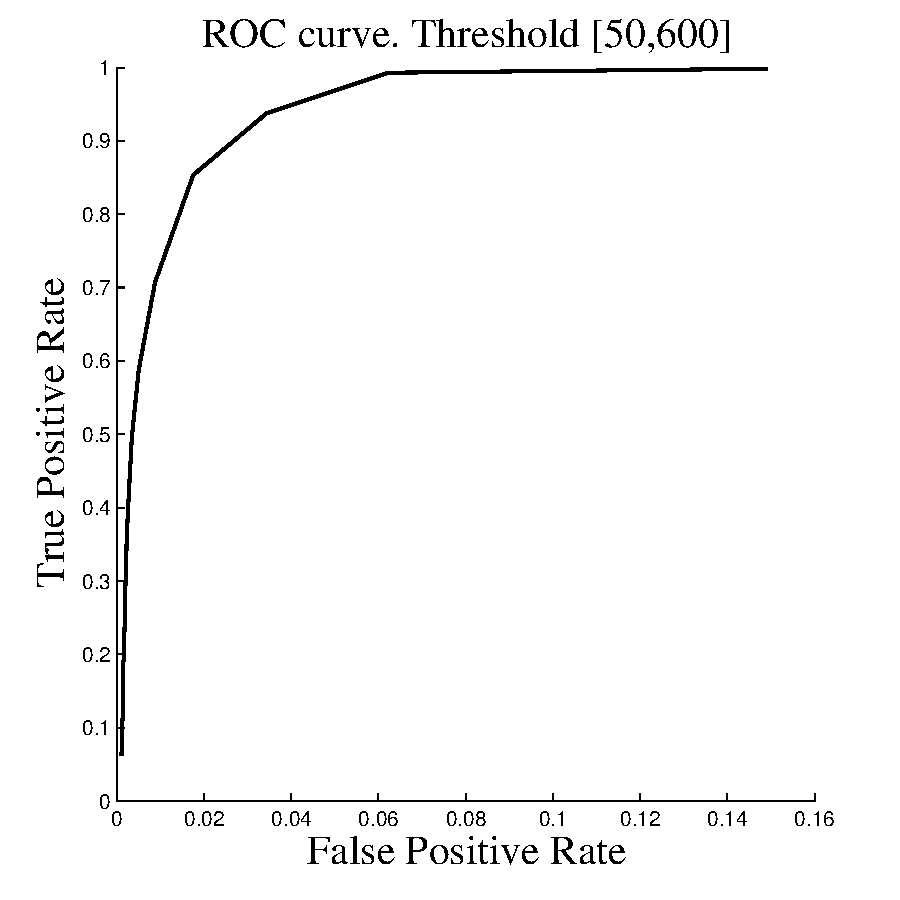
\includegraphics[width=0.25\textwidth]{Figures/ROC_StarAsteroid_130_pchip_f20.pdf} &\includegraphics[width=0.25\textwidth]{Figures/ROC_Triplets_130_pchip_f20.pdf} 
\end{array}$
\end{center}
\vspace{-0.7cm}
\caption{Left: ROC curve for the detection of stars and asteroids after the Image thresholding stage of the pipeline. Right:  ROC curve for asteroid detections at the final stage of the pipeline.}
\label{fig:ROC}
\vspace{-0.6cm}
\end{figure} 



\subsection{Simulated Space-Based Imagery}
\label{ssec:simulated}

Using RCE, asteroids are  modeled as spherical blackbody-like emitters, 
%(emissivity is less than 1)
with a cross-sectional area that approximates the sizes of actual asteroids and surface temperatures typical of sun-illuminated asteroids in an Earth-like orbit.  Similar to the way stars are modeled, the radiation emitted is modeled using a form of Planck's equation:

\vspace{-0.3cm}
\begin{equation}
\label{eq:Planck}
B_\lambda(T)= \epsilon	\frac{2hc^2}{\lambda^5} \frac{1}{e^{\frac{hc}{\lambda k_BT}} - 1}
\end{equation}
%\vspace{-0.04cm}
 where $B_\lambda(T)$ is the spectral radiance at a given wavelength $\lambda$ and temperature $T$ %(which in SI units would be $Wm^{-2} m^{-1}$). 
 The value $\epsilon$ is the emissivity of the asteroid, which essentially converts the blackbody spectral radiance into spectral irradiance. The constant, $h$ is the Planck's constant, $c$ is the speed of light, $\lambda$ is wavelength, $k_B$ is the Boltzmann constant, and $T$ is the temperature. 
 
 The asteroids are assumed to have a nominal temperature of 200 K due to solar heating and emissivities in the range from 0.9 to 0.98. 
 %Therefore, their spectral radiance would look like what is shown in Figure \ref{}(TODO: Add this figure? The plot in the year end report does not have the axes labeled.).  For this 200 K blackbody, the peak in the radiance occurs at a wavelength of 14.5 µm.
 The RCE uses stellar data available as part of the Two Micron All Sky Survey (2MASS), a stellar survey that scanned the entire sky in three IR bands (centered at 1.25 \textmu m, 1.65 \textmu m, and 2.17 \textmu m, respectively).  The 2MASS catalog also incorporates data in two visible bands from other surveys. 
 %
 An example of the simulated MWIR image and the ground truth trajectory derived from one set of simulated imagery is shown in Fig. \ref{Simulated_Image}. 
 %In this figure, the simulated images are super-imposed in order to visualize the asteroid trajectory in a single image. 
 %
 Fig. \ref{Trajectories_Sim} shows the final trajectories detected by our algorithm for one triplet and one quadruplet of the simulated MWIR dataset. As is shown in Fig. \ref{Trajectories_Sim}, using trajectory verification on a greater number of images in the sequence allows us to quickly disambiguate and reject false trajectories. In this case this trend is readily apparent when going from a triplet to a quadruplet of images.
%

We characterize the algorithm with regard to detections at each of the following three successive stages: the initial detection of objects, the detection of moving objects and the detection of trajectories.
In Fig.~\ref{num_detect}, we plot the number of detected objects at each step of the pipeline for each selected threshold value. We can verify that the number of detections monotonically decreases when the threshold increases. Note that we have found that this not always the case, especially since a higher number of detections at the thresholding stage may induce more cancellations at the logical differencing. Additionally, we note in the right plot in Fig.~\ref{num_detect} that the use of quadruplets allows for a single trajectory to be found irrespective of the value of the threshold used (and hence the number of detections found at the first stage), echoing the results displayed in Fig.~\ref{Trajectories_Sim}.
%
Last, we show the Receiver Operating Characteristic (ROC) for simulated space-based imagery in Fig.~\ref{fig:ROC}.  
%
%Results for each step of the pipeline are shown:
% Image Registration in Figure~\ref{}. Logical differencing in Figure~\ref{}. (See Figure ~\ref{} for trajectory detection on an example image triplet).    As is shown in Figure~\ref{}, using trajectory verification on a greater number of images in the sequence allows us to quickly disambiguate and reject false trajectories (in this case this trend is readily apparent when going from a triplet to a quadruplet of images).

\subsection{Real Imagery}

\subsubsection{NEAT}
Near Earth Asteroid Tracking (NEAT)~\cite{neat2014} is an earth-based program run by NASA from 1995-2007 to discover NEOs.
Fig. \ref{IPP_NEAT_Layout1} and Fig. \ref{fig:IPP_NEAT_Trajectory} show the results at all stages of the pipeline for one triplet of images of the 2002-CY46 asteroid obtained from the NEAT system archive. 
%The following figures show the results at all stages of the pipeline for one triplet of images of the 2002-CY46 asteroid obtained from the NEAT \cite{neat2014} survey. 
 
%\begin{figure*}
%\minipage{0.33\textwidth}
%  \includegraphics[width=\linewidth]{Figures/NEAT1.pdf}
%\endminipage\hfill
%\minipage{0.33\textwidth}
%  \includegraphics[width=\linewidth]{Figures/NEAT2.pdf}
%\endminipage\hfill
%\minipage{0.33\textwidth}
%  \includegraphics[width=\linewidth]{Figures/NEAT3.pdf}
%\endminipage
%\caption{2002 CY46 Triplet Near Earth Asteroid Tracking (NEAT) system archive}
%\label{fig:NEAT_Images}
%\end{figure*}
\vspace{-0.2cm}
\newcommand{\imgWidth}{0.15\textwidth}
\begin{figure}[h]
\begin{center}$
\begin{array}{@{\hspace{0.2em}}c@{\hspace{0.3em}}c@{\hspace{0.3em}}c}
\includegraphics[width=\imgWidth]{Figures/NEAT1.pdf} &
\includegraphics[width=\imgWidth]{Figures/NEAT2.pdf} &
\includegraphics[width=\imgWidth]{Figures/NEAT3.pdf} \\
\includegraphics[width=\imgWidth]{Figures/NEATImageReg12.pdf} &
\includegraphics[width=\imgWidth]{Figures/NEAT2.pdf} &
\includegraphics[width=\imgWidth]{Figures/NEATImageReg32.pdf} \\
\includegraphics[width=\imgWidth]{Figures/NEATImageDiff1.pdf} &
\includegraphics[width=\imgWidth]{Figures/NEATImageDiff2.pdf} &
\includegraphics[width=\imgWidth]{Figures/NEATImageDiff3.pdf} \\
\includegraphics[width=\imgWidth]{Figures/NEATFilteredCentroids1.pdf} &
\includegraphics[width=\imgWidth]{Figures/NEATFilteredCentroids2.pdf} &
\includegraphics[width=\imgWidth]{Figures/NEATFilteredCentroids3.pdf}
\end{array}$
\end{center}
\vspace{-0.7cm}
\caption[caption]{Image Processing Pipeline results shown on 2002 NEAT data. 
(row 1):  input image triplet (CY46) taken approx. 10 minutes apart. 
(row 2): Image Registration. Left: Image-1 registered to Image-2. Right: Image-3 registered to Image-2. 
%\\\hspace{\textwidth} 
(row 3): Image Differencing: Artifacts such as crater-like formations are seen in the difference images above. This is the result of some celestial bodies being over-exposed.) 
%\\\hspace{\textwidth} 
(row 4): Image Differencing: Filtered centroids shown in each image of the sequence.)}
\label{IPP_NEAT_Layout1}
\end{figure}

\begin{figure}[!]
%\minipage{0.40\textwidth}
%  \includegraphics[width=\linewidth]{Figures/NEATLines_LogicalImg.pdf}
%\endminipage\hfill
\vspace{-0.25cm}
\begin{center}
\includegraphics[width=0.3\textwidth]{Figures/NEATLines_LogicalImg.pdf}
\end{center}
\vspace{-0.7cm}
\caption{Trajectory Detection for the NEAT CY46 Triplet. Asteroid trajectory detected is shown in green. True location is in red. 3 Images of the triplet are super-imposed here after registration and thresholding for ease of visualization.}
\label{fig:IPP_NEAT_Trajectory}
\vspace{-0.3cm}
\end{figure}

%\begin{figure}[h]
%\vspace{-0.1cm}
%\begin{center}
%\includegraphics[width=0.3\textwidth]{Figures/CSS_Quad_Black_Lines.pdf} 
%\end{center}
%\vspace{-0.7cm}
%\caption[caption]{Image Processing results shown on Catalina Sky Survey data.}
%%\\\hspace{\textwidth} 
%\label{IPP_Catalina_Layout2}
%\end{figure}

\begin{figure}[h]
\begin{center}$
\begin{array}{@{\hspace{-0.7em}}c@{\hspace{0.2em}}c@{\hspace{0.2em}}}
\includegraphics[width=0.25\textwidth]{Figures/CSS_Triplet_Lines_Dark.pdf} &\includegraphics[width=0.25\textwidth]{Figures/CSS_Quad_Lines.pdf} 
\end{array}$
\end{center}
\vspace{-0.7cm}
\caption{Image Processing results shown on CSS data.The registered images are super-imposed to visualize the trajectory in a single image.Asteroid trajectory detected is shown in green, true location is in red. Left: Trajectories detected on a triplet. Right: Trajectory detected on a quadruplet.}
\label{IPP_Catalina_Layout1}
\vspace{-0.6cm}
\end{figure} 

%
%\begin{figure}[t]
%\vspace{-0.7cm}
%\begin{center}$
%\begin{array}{@{\hspace{0.2em}}c@{\hspace{0.3em}}c@{\hspace{0.3em}}c}
%\includegraphics[width=\imgWidth]{Figures/CSS_100_5000_1.pdf} &
%\includegraphics[width=\imgWidth]{Figures/CSS_100_5000_2.pdf} &
%\includegraphics[width=\imgWidth]{Figures/CSS_100_5000_3.pdf} \\
%\includegraphics[width=\imgWidth]{Figures/ImageReg12_CSS.pdf} &
%\includegraphics[width=\imgWidth]{Figures/CSS_100_5000_2.pdf} &
%\includegraphics[width=\imgWidth]{Figures/ImageReg32_CSS.pdf} \\
%\includegraphics[width=\imgWidth]{Figures/ImageDiff_CSS1.pdf} &
%\includegraphics[width=\imgWidth]{Figures/ImageDiff_CSS2.pdf} &
%\includegraphics[width=\imgWidth]{Figures/ImageDiff_CSS3.pdf} 
%\end{array}$
%\end{center}
%\vspace{-0.7cm}
%\caption[caption]{Image Processing Pipeline results shown on Catalina Sky Survey data. 
%(row 1):  input image triplet taken approx. 10 minutes apart. 
%(row 2): Image Registration. Left: Image-1 registered to Image-2. Right: Image-3 registered to Image-2. 
%%\\\hspace{\textwidth} 
%(row 3): Image Differencing results }
%%\\\hspace{\textwidth} 
%\label{IPP_Catalina_Layout1}
%\end{figure}



%\begin{figure}[h]
%%\minipage{0.40\textwidth}
%%  \includegraphics[width=\linewidth]{Figures/NEATLines_LogicalImg.pdf}
%%\endminipage\hfill
%\vspace{-0.7cm}
%\begin{center}
%\includegraphics[width=0.4\textwidth]{Figures/NEATLines_LogicalImg.pdf}
%\end{center}
%\vspace{-0.7cm}
%\caption{Trajectory Detection for the CSS Triplet. Asteroid trajectory detected is shown in green. True location is in red. 3 Images of the triplet are super-imposed here after registration and thresholding for ease of visualization.}
%\label{fig:IPP_CSS_Trajectory}
%\vspace{-0.3cm}
%\end{figure}

\newcommand{\imgWidthMedium}{0.23\textwidth}
\begin{figure*}[h]
\begin{center}$
\begin{array}{c@{\hspace{.5em}}c@{\hspace{0.5em}}c@{\hspace{0.5em}}c}
\includegraphics[width=\imgWidthMedium]{Figures/NEAT1.pdf} &
\includegraphics[width=\imgWidthMedium]{Figures/NEATImageReg12.pdf} &
\includegraphics[width=\imgWidthMedium]{Figures/NEATImageDiff1.pdf} &
\includegraphics[width=\imgWidthMedium]{Figures/NEATFilteredCentroids1.pdf} \\
\includegraphics[width=\imgWidthMedium]{Figures/NEAT2.pdf} &
\includegraphics[width=\imgWidthMedium]{Figures/NEATImageReg22.pdf} &
\includegraphics[width=\imgWidthMedium]{Figures/NEATImageDiff2.pdf} &
\includegraphics[width=\imgWidthMedium]{Figures/NEATFilteredCentroids2.pdf} \\
\includegraphics[width=\imgWidthMedium]{Figures/NEAT3.pdf} &
\includegraphics[width=\imgWidthMedium]{Figures/NEATImageReg32.pdf} &
\includegraphics[width=\imgWidthMedium]{Figures/NEATImageDiff3.pdf} &
\includegraphics[width=\imgWidthMedium]{Figures/NEATFilteredCentroids3.pdf} 
\end{array}$
\end{center}
\vspace{-0.7cm}
\caption[caption]{Image Processing Pipeline results for the CY46 Triplet. (column 1): 2002 CY46 Triplet images taken approximately 10 minutes apart. Near Earth Asteroid Tracking (NEAT) system archive. 
%\\\hspace{\textwidth} 
(column 2): Image Registration results for the CY46 Triplet.  Top: Image-1 registered to Image-2. Middle: Image-2 Bottom: Image-3 registered to Image-2. 
(column 3): Image Differencing results for the CY46 Triplet. (Artifacts such as crater-like formations are seen in the difference images above. This is the result of some celestial bodies being over-exposed.) 
(column 4): Image Differencing results for the CY46 Triplet. Filtered centroids in each image of the sequence.)}
\label{IPP_NEAT_Layout2}
\end{figure*}

%\begin{figure*}[h]
%\begin{center}$
%\begin{array}{ccc}
%\includegraphics[width=0.33\textwidth]{Figures/NEAT1.pdf} &
%\includegraphics[width=0.33\textwidth]{Figures/NEAT2.pdf} &
%\includegraphics[width=0.33\textwidth]{Figures/NEAT3.pdf} \\
%\includegraphics[width=0.33\textwidth]{Figures/NEATImageReg12.pdf} &
%\includegraphics[width=0.33\textwidth]{Figures/NEATImageReg22.pdf} &
%\includegraphics[width=0.33\textwidth]{Figures/NEATImageReg32.pdf} \\
%\includegraphics[width=0.33\textwidth]{Figures/NEATImageDiff1.pdf} &
%\includegraphics[width=0.33\textwidth]{Figures/NEATImageDiff2.pdf} &
%\includegraphics[width=0.33\textwidth]{Figures/NEATImageDiff3.pdf} \\
%\includegraphics[width=0.33\textwidth]{Figures/NEATFilteredCentroids1.pdf} &
%\includegraphics[width=0.33\textwidth]{Figures/NEATFilteredCentroids2.pdf} &
%\includegraphics[width=0.33\textwidth]{Figures/NEATFilteredCentroids3.pdf}
%\end{array}$
%\end{center}
%\caption[caption]{Image Processing Pipeline results for the CY46 Triplet. 
%First row: 2002 CY46 Triplet images taken approximately 10 minutes apart. Near Earth Asteroid Tracking (NEAT) system archive. \\\hspace{\textwidth} 
%Second row: Image Registration results for the CY46 Triplet.  Top: Image-1 registered to Image-2. Middle: Image-2 Bottom: Image-3 registered to Image-2.
%\\\hspace{\textwidth}
%Third row: Image Differencing results for the CY46 Triplet. (Artifacts such as crater-like formations are seen in the difference images above. This is the result of some celestial bodies being over-exposed.) 
%\\\hspace{\textwidth}
%Fourth row: Image Differencing results for the CY46 Triplet. Filtered centroids in each image of the sequence.)}
%\label{IPP_NEAT_Layout3}
%\end{figure*}

%\begin{figure}[b]
%\minipage{0.24\textwidth}
%  \includegraphics[width=\linewidth]{Figures/NEATImageReg12.pdf}
%\endminipage\hfill
%\minipage{0.24\textwidth}
%  \includegraphics[width=\linewidth]{Figures/NEATImageReg32.pdf}
%\endminipage\hfill
%\caption{Image Registration results for the CY46 Triplet.  Left: Image-1 registered to Image-2. Right: Image-3 registered to Image-2.}
%\label{fig:NEAT_Registration}
%\end{figure}

%\begin{figure*}
%\minipage{0.33\textwidth}
%  \includegraphics[width=\linewidth]{Figures/NEATImageDiff1.pdf}
%\endminipage\hfill
%\minipage{0.33\textwidth}
%  \includegraphics[width=\linewidth]{Figures/NEATImageDiff2.pdf}
%\endminipage\hfill
%\minipage{0.33\textwidth}
%  \includegraphics[width=\linewidth]{Figures/NEATImageDiff3.pdf}
%\endminipage
%\caption{Image Differencing results for the CY46 Triplet. (Artifacts such as crater-like formations are seen in the difference images above. This is the result of some celestial bodies being over-exposed.)}
%\label{fig:NEAT_ImgDiff1}
%\end{figure*}

%\begin{figure*}
%\minipage{0.33\textwidth}
%  \includegraphics[width=\linewidth]{Figures/NEATFilteredCentroids1.pdf}
%\endminipage\hfill
%\minipage{0.33\textwidth}
%  \includegraphics[width=\linewidth]{Figures/NEATFilteredCentroids2.pdf}
%\endminipage\hfill
%\minipage{0.33\textwidth}
%  \includegraphics[width=\linewidth]{Figures/NEATFilteredCentroids3.pdf}
%\endminipage
%\caption{Image Differencing results for the CY46 Triplet. Filtered centroids in each image of the sequence.)}
%\label{fig:NEAT_ImgDiff2}
%\end{figure*}

\vspace{-0.7cm}
\subsubsection{CATALINA}
The Catalina Sky Survey (CSS) \cite{larson1998catalina,drake2009first} is intended to discover NEOs, specifically potentially hazardous asteroids that pose risk to earth. Fig. \ref{IPP_Catalina_Layout1} 
%and Fig. \ref{fig:IPP_CSS_Trajectory} 
shows the final result for one set of earth-based images from CSS.
\vspace{-0.3cm}
\subsection{Implementation}
This pipeline has been developed and tested in MATLAB and has also been jointly implemented in C++ on a recent Intel processor. Preliminary benchmarking on this processor has shown that peak memory usage is of the order 92 MB. Additional preliminary studies for extrapolating CPU and memory usage on an MCP750 -- a good proxy for BAE's RAD750, an operational spacecraft processor -- have led to metrics that seem promising for a possible deployment on a spacecraft architecture. We are now conducting additional work to validate these figures including activities involving the deployment of this algorithm onto a  MCP750  in conjunction with FPGAs. 

